% We switch to portrait mode. This works as advertised.
\documentclass[xcolor=table]{beamer}
\usepackage[orientation=portrait, size=a0, scale=1]{beamerposter}

\usepackage[utf8]{inputenc}
\usepackage[british]{babel}
\usepackage[super]{nth}

%math
\usepackage{amsmath,mathtools}
\usepackage{amssymb}

%chemistry
\usepackage[version=3]{mhchem}
\usepackage{chemfig}
\usepackage{setspace}

%physics
\usepackage[separate-uncertainty = true]{siunitx}

%\usetheme{Boadilla}
%\usecolortheme{rose}
%\usecolortheme{crane}
%\usefonttheme{structuresmallcapsserif}
%\setbeamertemplate{navigation symbols}{}

\mode<presentation>{\usetheme{ilm}}

%\definecolor{Main}{rgb}{0.74, 0.13, 0.19}
\colorlet{Main}{ilmorange}
%\definecolor{Accent1}{rgb}{0.76,0.36,0.13}
\colorlet{Accent1}{ilmcolor}
%\definecolor{Accent2}{rgb}{0.54,0.1,0.4}
\colorlet{Accent2}{ilmcolor!65!black}



% see documentation for a0poster class for the size options here
\let\Textsize\normalsize
\def\Norulehead#1{\noindent\hbox to \hsize{\hfil\LARGE\textcolor{Main}{\textbf{#1}}}\bigskip}
\def\Head#1{\Norulehead{\hrulefill #1}}
\def\LHead#1{\noindent{\Large \color{Accent2}\textbf{#1}}\smallskip}
\def\affiliation#1{\Large \textcolor{Accent2}{\textit{#1}}\smallskip}
\def\Subhead#1{\noindent{\large\color{Accent1}\textbf{#1}}}
\def\Title#1{\noindent{\veryHuge\color{Main}\raggedright\textsf{\textbf{#1}}}}

\setbeamertemplate{headline}{%
	%logo sponsors
	\let\mydim\relax
	\newlength\mydim
	\setlength{\mydim}{0.75cm}
	\rule[-.3\baselineskip]{0pt}{4.5cm}
	\hfill\pgfuseimage{cnrs-logo}\hspace*{\mydim}\pgfuseimage{ucbl-logo}\hspace*{\mydim}
	
\includegraphics[height=3cm]{presentation/ENS_Lyon.pdf}\hspace*{\mydim}
	\pgfuseimage{univlyon-logo}\hspace*{\mydim}
	
\includegraphics[height=4cm]{presentation/invest-avenir.pdf}\hspace*{\mydim}
	\includegraphics[height=4cm,clip=true, trim=6mm 14mm 6mm 0]{../Yaourt/NEW-Logo-ERC-OUTLINE}\hspace*{\mydim}
	
\includegraphics[height=3cm]{presentation/frama.png}\hspace*{\mydim}
	
\includegraphics[height=4cm]{presentation/ICL}\hspace*{\mydim}
}

% The textpos package is necessary to position textblocks at arbitary 
% places on the page.
\usepackage[absolute,overlay,showboxes
]{textpos}
% Set up the grid
%
% Note that [40mm,40mm] is the margin round the edge of the page --
% it is _not_ the grid size. That is always defined as 
% PAGE_WIDTH/HGRID and PAGE_HEIGHT/VGRID. In this case we use
% 15 x 25. This gives us a wide central column for text (7 grid
% spacings) and two narrow columns (3 each) at each side for 
% pictures, separated by 1 grid spacing.
%
% Note however that texblocks can be positioned fractionally as well,
% so really any convenient grid size can be used.
%
\TPGrid[40mm,40mm]{15}{25}  % 3 - 1 - 7 - 1 - 3 Columns

% Mess with these as you like
\parindent=0pt
%\parindent=1cm
\parskip=0.5\baselineskip

\usepackage{paralist}
\usepackage{tabu}

% Allow the usage of graphics (.jpg, .png, etc.) in the document
\usepackage{graphicx}
\usepackage{tikz}
\usetikzlibrary{arrows,shapes,backgrounds, calc, positioning, topaths,chains, intersections, decorations.markings, decorations.text, shapes.geometric, matrix,patterns,mindmap,fit}
%\usetikzlibrary{positioning, patterns,topaths,chains,matrix}

\usepackage{pgfplots}
\usepackage{pgfplotstable}
\pgfplotsset{compat=1.9}
\usepgfplotslibrary{fillbetween}
\usepgfplotslibrary{groupplots}
\usepgfplotslibrary{external}
\makeatletter
\newcommand*{\overlaynumber}{\number\beamer@slideinframe}
\tikzset{
  beamer externalizing/.style={%
    execute at end picture={%
      \tikzifexternalizing{%
        \ifbeamer@anotherslide
        \pgfexternalstorecommand{\string\global\string\beamer@anotherslidetrue}%
        \fi
      }{}%
    }%
  },
  external/optimize=false
}
\let\orig@tikzsetnextfilename=\tikzsetnextfilename
\renewcommand\tikzsetnextfilename[1]{\orig@tikzsetnextfilename{#1-\overlaynumber}}
\makeatother

%\tikzset{every picture/.style={beamer externalizing}}
%\tikzexternalize
%\tikzsetexternalprefix{fig_poster/}



\begin{document}
\begin{frame}
%title
\begin{textblock}{15}(0,0.8)

{\setlength{\baselineskip}{2.75\baselineskip}\hspace*{0.3\paperwidth}\Title{
Ion pairing controls rheological properties of ``processionary'' polyelectrolyte hydrogels
}\hfill \textit{Soft Matter} 2016, \textbf{12}, 9749-9758\par}

\centering

\vspace{0.5cm}
\LHead{Hassan Srour,\textit{$^{1}$} Martien Duvall Deffo Ayagou,\textit{$^{1}$} Thi Thanh-Tam Nguyen,\textit{$^{1}$}, Nicolas Taberlet,\textit{$^{2}$} S\'{e}bastien Manneville,\textit{$^{2}$}\\ Chantal Andraud,\textit{$^{1}$} Cyrille Monnereau,$^{\ast}$\textit{$^{1}$} and Mathieu Leocmach$^{\ast}$\textit{$^{3}$
}}\hspace{0.1\paperwidth}\texttt{\color{Main}\Large mathieu.leocmach@univ-lyon1.fr}\\

\affiliation{$^{1}$ Univ Lyon, Ens de Lyon, Universit\'e Claude Bernard Lyon 1, CNRS,
Laboratoire de Chimie, F-69342 Lyon, France.\\
$^{2}$ Univ Lyon, Ens de Lyon, Universit\'e Claude Bernard Lyon 1, CNRS,
Laboratoire de Physique, F-69342 Lyon, France.\\
$^{3}$ Univ Lyon, Universit\'e Claude Bernard Lyon 1, CNRS, Institut Lumi\`ere Mati\`ere, F-69622, VILLEURBANNE}
\end{textblock}%title


\begin{textblock}{4}(0,4)
	\Head{Cation terminated polyanion}
	\tikzsetnextfilename{polymerisation}%
	\let\mrad\relax%
	\newlength\mrad%
	\setlength{\mrad}{1ex}%
	% The face style, can be changed
	\tikzset{face/.style={
		shape=circle,minimum size=2\mrad,shading=radial,outer sep=0pt,
	    inner color=white!50!yellow,outer color= yellow!70!orange
		}}%
	\begin{tikzpicture}
		\foreach \i [evaluate=\i as \dist using \i*0.45] in {0,1,2}{
			\begin{scope}[xshift=\dist\textwidth]
			%face
			\begin{scope}[face/.style={
		shape=circle,minimum size=2\mrad,shading=radial,outer sep=0pt,
	    inner color=white!50!yellow,outer color= yellow!70!orange
		}]
\node[face,inner color=white!50!ilmcolor,outer color= ilmcolor!90!black] (emoticon) {};
			%% The eyes are fixed.
			\draw[fill=white] 
				(-0.5\mrad,0ex) ..controls (-0.25\mrad,0.1\mrad)and(0.25\mrad,0.1\mrad)..
		        (0.5\mrad,0.0pt) ..controls (0.75\mrad,0.75\mrad)and(0.1\mrad,0.85\mrad)..
		        (0pt,0.2\mrad) ..controls (-0.1\mrad,0.85\mrad)and(-0.75\mrad,0.75\mrad)..
		        (-0.5\mrad,0pt)--cycle;
			%% standard pupils
			\node[fill, ellipse,inner xsep=0.075\mrad, inner ysep=0.0375\mrad, rotate=80] at (0.25\mrad,0.25\mrad) {};
			\node[fill, ellipse,inner xsep=0.075\mrad, inner ysep=0.0375\mrad, rotate=100] at (-0.25\mrad,0.25\mrad) {};
			%% mouth
			\draw[thick,line cap=round] (-0.5\mrad,-0.5\mrad)
			     ..controls (-0.25\mrad,-0.75\mrad)and(0.25\mrad,-0.75\mrad)..(0.5\mrad,-0.5\mrad);
\end{scope}
;
			%% horns
			\draw[every node/.style={shape=circle,inner sep=0.2\mrad,shading=radial,inner color=white!50!ilmcolor,outer color= ilmcolor!90!black}] (emoticon.70) -- ++(70:0.4\mrad) node{} (emoticon.110) -- ++(110:0.4\mrad) node{};
			%\draw ( emoticon.80)..controls ( 0.3\mrad,1.2\mrad)..(0.5\mrad,1.25\mrad)
			      %..controls ( 0.4\mrad,1.15\mrad)..(emoticon.70);
			%\draw (emoticon.100)..controls (-0.3\mrad,1.2\mrad)..(-0.5\mrad,1.25\mrad)
			      %..controls (-0.4\mrad,1.15\mrad)..(emoticon.110);
			%body segments
			\ifthenelse{\i=0}{}{
			\foreach \x in {0,2,...,10}{
				\node[face,inner color=white!50!gray,outer color= gray!90!black, left=\x\mrad of emoticon] (monomer){};
				%legs
				\ifthenelse{\i=1}{}{
					\draw[line width=0.25\mrad, ilmorange] (monomer.south) ++(0,0.5\mrad) to[bend left] +(0,-1\mrad);}
			};}
			\ifthenelse{\i=1}{
				\draw[|-|] ($(monomer.west)+(0,-1.5\mrad)$) -- ($(emoticon.west)+(0,-1.5\mrad)$) node[midway,below, font=\scriptsize] {$N_0$};
			}{}
			\end{scope}
			};
			%arrows
			\draw[-stealth, thick] ++(3\mrad,0) -- +(6\mrad,0) node[midway, above=0.2\mrad, face,inner color=white!50!gray,outer color= gray!90!black]{} node[midway, below, font=\scriptsize]{ATRP};
			\draw[-stealth, thick] ++(0.45\textwidth,0) ++(3\mrad,0) -- +(6\mrad,0) coordinate[midway, above=0.2\mrad] (leg) node[midway, below, font=\scriptsize,text width=10\mrad,align=center]{post-functionalization};
			\draw[line width=0.25\mrad, ilmorange] (leg) to[bend right] +(0,1\mrad);
		\end{tikzpicture}

	\bigskip
	\tikzsetnextfilename{polymerisation_PImBr}%
	\definesubmol{head}{(-[::-105,,,,ilmcolor])(-[::-15,,,,ilmcolor])-[::60,,,,ilmcolor](=[::60,,,,ilmcolor]\textcolor{ilmcolor}{O})-[::-60,,,,ilmcolor]\textcolor{ilmcolor}{O}-[::-60,,,,ilmcolor]-[::60,,,,ilmcolor]-[::60,,,,ilmcolor]}
\definesubmol{mono}{-[::-60,,,,gray](=[,,,,gray]\textcolor{gray}{O})-[::-60,,,,gray]\textcolor{gray}{O}-[::60,,,,gray]-[,,,,gray]-[::-60,,,,gray]}
\tikzsetnextfilename{polymerisation_PImBr}
\begin{tikzpicture}[every node/.style={font=\tiny\setatomsep{1.5em}}]
	\node (init) {\chemfig{Br-[:-30]!{head}\textcolor{ilmcolor}{P}|\textcolor{ilmcolor}{O_3}Et_2}};
	
	\node[below left=5\baselineskip and 0 of init.east] (POH) {%
	\chemfig{[:-30]-[@{left,0.25}](%
		!{mono}OH%
		)-[::60,,,,gray]-[@{right,0.25}]!{head}\textcolor{ilmcolor}{P}|\textcolor{ilmcolor}{O_3}Et_2}%
	};
	\node[below right=-0.6em and -0.25em of POH.base west] {$\prescript{}{N_0}{\left[\vrule height 1em depth 0.25em width 0pt\hspace{1.75em}\right]}$};
	\node[below right=-0.6em and -0.25em of POH.base west] {};
	
	\node[right=0.1\textwidth of init.base east, anchor=base west] (PBr) {%
	\chemfig{[:-30]-[@{left,0.25}](%
		!{mono}Br%
		)-[::60,,,,gray]-[@{right,0.25}]!{head}\textcolor{ilmcolor}{P}|\textcolor{ilmcolor}{O_3^{2-}}}%
	};
	\node[below right=-0.6em and -0.25em of PBr.base west] {$\prescript{}{N_0}{\left[\vrule height 1em depth 0.25em width 0pt\hspace{1.75em}\right]}$};
	
	\node[right=\textwidth of init.base-|POH.west, anchor=base east] (PNuBr) {%
	\chemfig{[:-30]-[@{left,0.25}](%
		!{mono}\textcolor{ilmorange}{N}|^{\color{ilmorange}+}*5(=[,,,,thick, ilmorange]-[,,,,thick, ilmorange]\textcolor{ilmorange}{N}(-[,,,,thick, ilmorange])-[,,,,thick, ilmorange]=[,,,,thick, ilmorange]-[,,,,thick, ilmorange])(-[0,2,,,draw=none]Br^{-})
		)-[::60,,,,gray]-[@{right,0.25}]!{head}\textcolor{ilmcolor}{P}|\textcolor{ilmcolor}{O_3^{2-}}}%
	};
	\node[below right=-0.6em and -0.25em of PNuBr.base west] {$\prescript{}{N_0}{\left[\vrule height 1em depth 0.25em width 0pt\hspace{1.75em}\right]}$};
	
	\draw[-stealth, thick] (init.south-|POH.north) -- (POH) node[midway, left=0, -]{\chemfig{[:-30]=[,,,,gray]!{mono}OH}} node[midway, right=0, text width=0.13\textwidth, align=center]{\ce{CuBr}\linebreak 4-4'-bipyridine\linebreak \SI{85}{\celsius}};
	\draw[-stealth, thick] (POH) -| (PBr) node[pos=0.25, above]{\ce{TMS-Br}} node[pos=0.25, below, sloped, text width=0.2\textwidth, align=center]{\ce{CH2Cl2}\linebreak \SI{85}{\celsius}};
	\draw[-stealth, thick] (PBr) -- (PBr-|PNuBr.west) node[midway, above,align=center,-]{\chemfig[thick, ilmorange]{[2]*5(-N(-)-=N-=)}} node[midway, below, text width=0.2\textwidth, align=center]{THF\linebreak \SI{85}{\celsius}};;
	\node[anchor=south east] at (POH.south east) {\ce{POH}};
	\node[anchor=south east] at (PBr.south east) {\ce{PBr}};
	\node[anchor=south east] at (PNuBr.south east) {\ce{PIm+Br-}};
	\node[anchor=south east, font=\footnotesize] at (POH.south-|PNuBr.east) {$N_0=70$ from NMR};
\end{tikzpicture}
\end{textblock} %synthesis

\begin{textblock}{3}(5,4)
\Head{Yield stress fluid}
\Subhead{Reversible gel}

Herschel-Bulkley law \hfill$\sigma =\sigma_c + A \dot{\gamma}^n$
\tikzsetnextfilename{flowcurves}%
\begin{tikzpicture}
    \let\mrad\relax%
	\newlength\mrad%
	\setlength{\mrad}{0.5em}%
% The face style, can be changed
	\tikzset{face/.style={
		shape=circle,minimum size=2\mrad,shading=radial,outer sep=0pt,
	    inner color=white!50!yellow,outer color= yellow!70!orange
		}}%
\let\drawcaterpillar\relax
\newcommand\drawcaterpillar{
			%face
			\begin{scope}[face/.style={
		shape=circle,minimum size=2\mrad,shading=radial,outer sep=0pt,
	    inner color=white!50!yellow,outer color= yellow!70!orange
		}]
\node[face,inner color=white!50!ilmcolor,outer color= ilmcolor!90!black] (emoticon) {};
			%% The eyes are fixed.
			\draw[fill=white] 
				(-0.5\mrad,0ex) ..controls (-0.25\mrad,0.1\mrad)and(0.25\mrad,0.1\mrad)..
		        (0.5\mrad,0.0pt) ..controls (0.75\mrad,0.75\mrad)and(0.1\mrad,0.85\mrad)..
		        (0pt,0.2\mrad) ..controls (-0.1\mrad,0.85\mrad)and(-0.75\mrad,0.75\mrad)..
		        (-0.5\mrad,0pt)--cycle;
			%% standard pupils
			\node[fill, ellipse,inner xsep=0.075\mrad, inner ysep=0.0375\mrad, rotate=80] at (0.25\mrad,0.25\mrad) {};
			\node[fill, ellipse,inner xsep=0.075\mrad, inner ysep=0.0375\mrad, rotate=100] at (-0.25\mrad,0.25\mrad) {};
			%% mouth
			\draw[thick,line cap=round] (-0.5\mrad,-0.5\mrad)
			     ..controls (-0.25\mrad,-0.75\mrad)and(0.25\mrad,-0.75\mrad)..(0.5\mrad,-0.5\mrad);
\end{scope}

			
%body segments
			\foreach \x in {0,2,...,4}{
				\node[face,inner color=white!50!gray,outer color= gray!90!black, left=\x\mrad of emoticon] (monomer){};
				%legs
				\draw[line width=0.25\mrad, ilmorange] (monomer.south) ++(0,0.5\mrad) to[bend left] +(0,-1\mrad);
			};
}
\begin{loglogaxis}[
	name=ax,
	width=\textwidth-5em,
	height=6\baselineskip,
	xlabel=$\dot\gamma\,(\si{\per\second})$,
	ylabel={$\sigma$ (\si{\pascal)}},
	clip marker paths=true,
	scale only axis,
	]
	\addplot+[mark=o, ilmcolor] table[x=shear_rate, y=shear_stress] {data/PO3-P60-Im+-0pc-02-06-14_8pcw_flow curve_down.txt} node[pos=0, font=\scriptsize, inner xsep=0, below left=1em and 0]{8\% wt};
	\addplot+[mark=square, ilmcolor!60!black] table[x=shear_rate, y=shear_stress] {data/PO3-P60-Im+-0pc-02-06-14_22pcw_flow curve_down.txt} node[pos=1, font=\scriptsize, inner xsep=0, above right=0.2em and -0.5em]{22\% wt};
	\addplot+[ilmorange] table[x=shear_rate, y=shear_stress,skip coords between index={0}{20}] {data/Et-P60-Im+-0pc-21-05-14_10pcw_flow_curve_down.txt} node[pos=0, font=\scriptsize, inner xsep=0, right=0.8em]{10\% wt};
	\addplot[domain=2e-2:5e2]{0.47+1.19*x^0.7};
	\addplot[domain=2e-2:5e2]{7.5+15.1*x^0.62};
\end{loglogaxis}

\begin{scope}[shift=(ax.north), yshift=-2\mrad, xshift=-\mrad]
			\drawcaterpillar
			%% horns
			\draw[every node/.style={shape=circle,inner sep=0.2\mrad,shading=radial,inner color=white!50!ilmcolor,outer color= ilmcolor!90!black}] (emoticon.70) -- ++(70:0.4\mrad) node{} (emoticon.110) -- ++(110:0.4\mrad) node{};
\end{scope}
\begin{scope}[shift=(ax.south), yshift=2\mrad, xshift=-\mrad]
			\drawcaterpillar
\end{scope}
\end{tikzpicture}


\vspace*{-\baselineskip}
\begin{columns}
\column{0.5\textwidth}
\begin{itemize}
	\item ionic strength, pH
	\item non ionic head
\end{itemize}
\column{0.4\textwidth}
\hfill$\Rightarrow$\hfill Solution
\end{columns}
$\Rightarrow$ Head-to-body ionic bonds

\vspace*{-0.5em}\textit{\footnotesize Srour et al. Macromol. Rapid Comm., 36, 55 (2015)}

\end{textblock} %Yield-stress fluid

\begin{textblock}{2}(9,4)
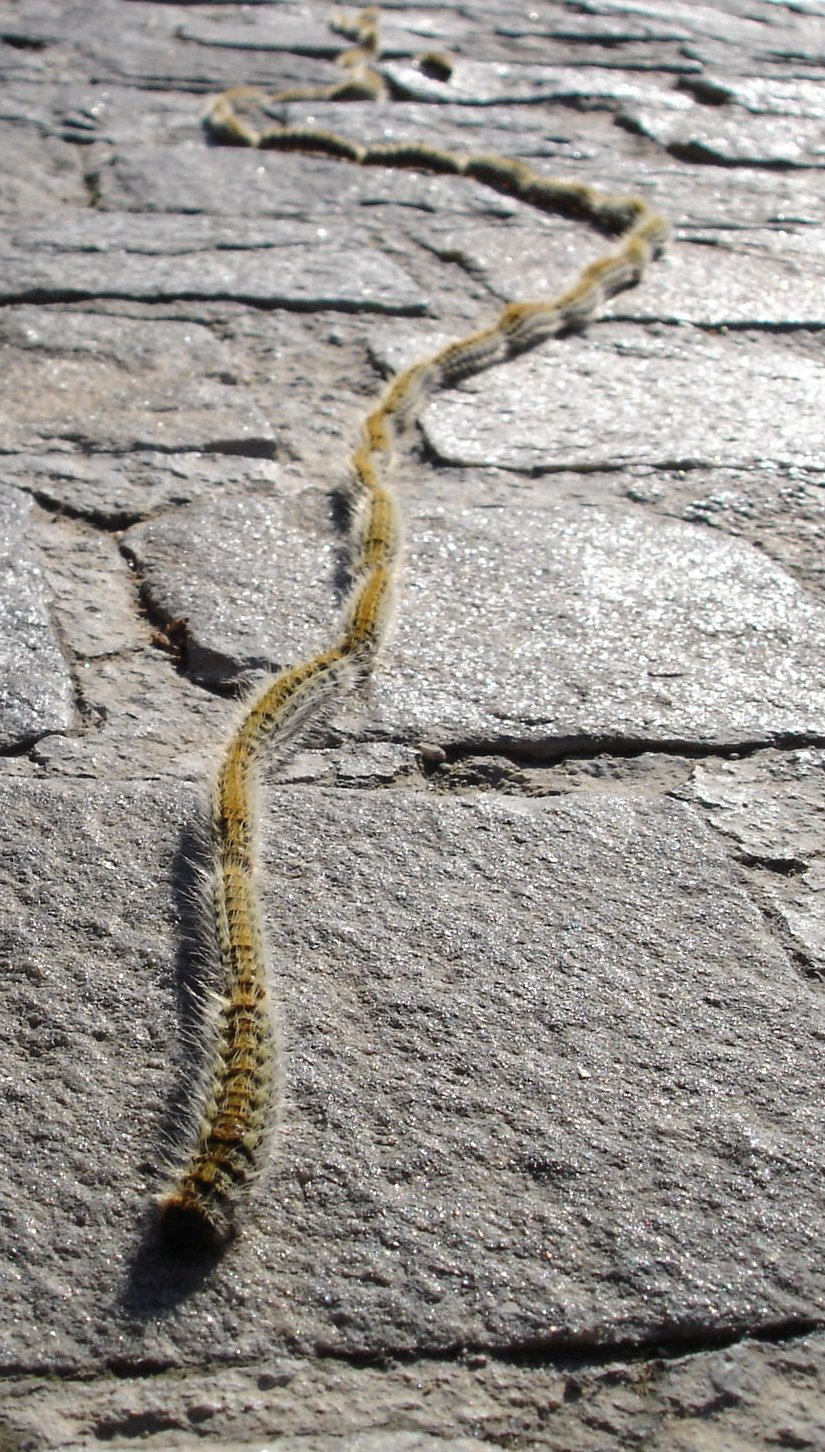
\includegraphics[width=\textwidth]{presentation/Thaumetopea_pityocampa_01.jpg}\\
	\vspace{-1.5em}\colorbox{lightgray}{\scriptsize Jürgen Appel on Wikimedia commons}
\end{textblock} %procession picture

\begin{textblock}{4}(0,8.25)
	\Head{Procession length}
	\[ G = \frac{c}{N}k_\mathrm{B}T \qquad \begin{array}{ll}
	\textcolor{Main}{c} & \text{monomer concentration}\\
	\textcolor{Main}{N} & \text{\# monomers between crosslinks}\\
	\end{array}\]
	
	$G\approx \SI{13}{\pascal}$\hfill$\Rightarrow$\hfill
	$N \approx 800 N_0$\hfill$\Rightarrow$\hfill
	800 chains between CL!
\end{textblock} %procession length

\begin{textblock}{10}(5,8.25)
	\Head{Counterion condensation \& solubility}
	\begin{tabu}{XX}
	All counterions condensed $\Rightarrow$ neutral $\Rightarrow$ not soluble&
	``Enough'' free counterions $\Rightarrow$ repulsion $\Rightarrow$ soluble\\
	\end{tabu}
	\tikzsetnextfilename{polyelectrolytes}%
	\begin{tikzpicture}
\let\mrad\relax%
\newlength\mrad%
\setlength{\mrad}{0.45em}%
\draw[every node/.style={circle,draw,font=\tiny, inner sep=0,minimum height=0.5em}] (0,0) --(30:\mrad) node[above right,ilmcolor](antenne){-} (0,0)--(-30:\mrad) node[below right,ilmcolor]{-} (0,0)--++(-180:\mrad)\foreach \x in {1,2,...,35}{--++(150:\mrad)node[above,ilmorange]{+} node[above=0.5em]{-}--++(-150:\mrad)node[below=0,ilmorange]{+} node[below=0.5em]{-}};

\begin{scope}[xshift=0.5\textwidth+2\mrad]
\clip (2\mrad,5\mrad) rectangle ++(-0.5\textwidth, -10\mrad);
\draw[every node/.style={circle,draw,font=\tiny, inner sep=0,minimum height=0.5em}] (0,0) --(30:\mrad) node[above right,ilmcolor](antenne){-} (0,0)--(-30:\mrad) node[below right,ilmcolor]{-} (0,0)--++(-180:\mrad)\foreach \x [evaluate=\x as \r using 1/(rnd+0.1), evaluate=\x as \rr using 1/(rnd+0.1)] in {1,2,...,35}{--++(150:\mrad)node[above,ilmorange]{+} node[above=\r\mrad]{-}--++(-150:\mrad)node[below=0,ilmorange]{+} node[below=\rr\mrad]{-}};
\end{scope}
\end{tikzpicture}%

\end{textblock} %condensation

\begin{textblock}{5}(0,10)
	\Head{Postfunctionalisation}
	\tikzsetnextfilename{postfunc}%
	\let\mrad\relax%
	\newlength\mrad%
	\setlength{\mrad}{1ex}%
	% The face style, can be changed
	\tikzset{face/.style={
		shape=circle,minimum size=2\mrad,shading=radial,outer sep=0pt,
	    inner color=white!50!yellow,outer color= yellow!70!orange
		}}%
	\begin{tikzpicture}
		\foreach \i [evaluate=\i as \dist using (floor(\i/2))*0.4, evaluate=\i as \ys using 1.5*(\i-2*floor(\i/2))] in {1,2,3,4,5}{
			\begin{scope}[xshift=\dist\textwidth, yshift=\ys\baselineskip]
			
			%face
			\begin{scope}[face/.style={
		shape=circle,minimum size=2\mrad,shading=radial,outer sep=0pt,
	    inner color=white!50!yellow,outer color= yellow!70!orange
		}]
\node[face,inner color=white!50!ilmcolor,outer color= ilmcolor!90!black] (emoticon) {};
			%% The eyes are fixed.
			\draw[fill=white] 
				(-0.5\mrad,0ex) ..controls (-0.25\mrad,0.1\mrad)and(0.25\mrad,0.1\mrad)..
		        (0.5\mrad,0.0pt) ..controls (0.75\mrad,0.75\mrad)and(0.1\mrad,0.85\mrad)..
		        (0pt,0.2\mrad) ..controls (-0.1\mrad,0.85\mrad)and(-0.75\mrad,0.75\mrad)..
		        (-0.5\mrad,0pt)--cycle;
			%% standard pupils
			\node[fill, ellipse,inner xsep=0.075\mrad, inner ysep=0.0375\mrad, rotate=80] at (0.25\mrad,0.25\mrad) {};
			\node[fill, ellipse,inner xsep=0.075\mrad, inner ysep=0.0375\mrad, rotate=100] at (-0.25\mrad,0.25\mrad) {};
			%% mouth
			\draw[thick,line cap=round] (-0.5\mrad,-0.5\mrad)
			     ..controls (-0.25\mrad,-0.75\mrad)and(0.25\mrad,-0.75\mrad)..(0.5\mrad,-0.5\mrad);
\end{scope}

			%% horns
			\draw[every node/.style={shape=circle,inner sep=0.2\mrad,shading=radial,inner color=white!50!ilmcolor,outer color= ilmcolor!90!black}] (emoticon.70) -- ++(70:0.4\mrad) node{} (emoticon.110) -- ++(110:0.4\mrad) node{};
			%\draw ( emoticon.80)..controls ( 0.3\mrad,1.2\mrad)..(0.5\mrad,1.25\mrad)
			      %..controls ( 0.4\mrad,1.15\mrad)..(emoticon.70);
			%\draw (emoticon.100)..controls (-0.3\mrad,1.2\mrad)..(-0.5\mrad,1.25\mrad)
			      %..controls (-0.4\mrad,1.15\mrad)..(emoticon.110);
			%body segments
			
			\foreach \x in {0,2,...,8}{
				\node[face,inner color=white!50!gray,outer color= gray!90!black, left=\x\mrad of emoticon] (monomer){};
				%legs
				\ifthenelse{\i=3}{
					\draw[line width=0.25\mrad, ilmorange] (monomer.south) ++(0,0.5\mrad) to[bend left] +(0,-1\mrad);}{}
				\ifthenelse{\i=2}{
					\node[circle, inner sep=0.3\mrad, fill=ilmorange] at (monomer.south){};}{}
				\ifthenelse{\i=5}{
					\draw[line width=0.25\mrad, blue!80!black] (monomer.south) ++(0,0.5\mrad) to[bend left] +(0,-1\mrad);}{}
				\ifthenelse{\i=4}{
					\node[circle, inner sep=0.3\mrad, fill=blue!80!black] at (monomer.south){};}{}
			};
			\end{scope}
			};
			%arrows
			%\draw[-stealth, thick] ++(3\mrad,0) -- +(6\mrad,0) node[midway, above=0.2\mrad, face,inner color=white!50!gray,outer color= gray!90!black]{} node[midway, below, font=\scriptsize]{ATRP};
			\draw[-stealth, thick] ++(3\mrad,1.5\baselineskip) -- +(6\mrad,0) coordinate[midway, above=0.2\mrad] (leg) node[midway, below, font=\scriptsize,text width=10\mrad,align=center]{post-functionalization};
			\draw[line width=0.25\mrad, ilmorange] (leg) to[bend right] +(0,1\mrad);
			\draw[-stealth, thick] ++(3\mrad,0) -- +(6\mrad,0) node[midway, below=0.2\mrad, circle, inner sep=0.3\mrad, fill=ilmorange] (leg){};
			\draw[-stealth, thick] ++(0.425\textwidth,0) ++(3\mrad,0.75\baselineskip) -- +(6\mrad,0) coordinate[midway, above=0.2\mrad] (leg) node[midway, above, font=\scriptsize]{counterion} node[midway, below, font=\scriptsize,text width=10\mrad,align=center]{exchange};
		\end{tikzpicture}
	
	\tikzsetnextfilename{solubility}%
	\begin{tikzpicture}
\pgfdeclarelayer{background}
\pgfdeclarelayer{foreground}
\pgfsetlayers{background,main,foreground}
\node (PBr) {PBr} [->, level distance=9em, font=\footnotesize] 
	child [grow=-20] {node(PImBr) {\ce{P\textcolor{ilmorange}{\ce{Im+}}\textcolor{blue!80!black}{\ce{Br-}}}} [level distance=5em]
		child[grow=-30] {node(PImF) {\ce{P\textcolor{ilmorange}{\ce{Im+}}\textcolor{blue!80!black}{\ce{F-}}}}} 
		child[grow=east] {node(PImCl) {\ce{P\textcolor{ilmorange}{\ce{Im+}}\textcolor{blue!80!black}{\ce{Cl-}}}}} 
		child[grow=west] {node(PImI) {\ce{P\textcolor{ilmorange}{\ce{Im+}}\textcolor{blue!80!black}{\ce{I-}}}}}} 
	child [grow=-160] {node(PPyrBr) {\ce{P\textcolor{ilmorange}{\ce{Pyr+}}\textcolor{blue!80!black}{\ce{Br-}}}} [level distance=5em]
		child[grow=-30] {node(PPyrF) {\ce{P\textcolor{ilmorange}{\ce{Pyr+}}\textcolor{blue!80!black}{\ce{F-}}}}} 
		child[grow=east] {node(PPyrCl) {\ce{P\textcolor{ilmorange}{\ce{Pyr+}}\textcolor{blue!80!black}{\ce{Cl-}}}}} 
		child[grow=west] {node(PPyrI) {\ce{P\textcolor{ilmorange}{\ce{Pyr+}}\textcolor{blue!80!black}{\ce{I-}}}}}};
\begin{pgfonlayer}{background}
	\draw[lightgray, line width=0.3em, -stealth,rounded corners] (PImI.south) -- (PImBr.south) node[pos=0, below right] {Hoffmeister} -- (PImCl.south) -- (PImF);
	\draw[lightgray, line width=0.3em, -stealth,rounded corners] (PPyrI.south) -- (PPyrBr.south) node[pos=0, below right] {Hoffmeister} -- (PPyrCl.south) -- (PPyrF);
	\draw[ilmorange!25, line width=0.3em, -stealth,rounded corners] (PPyrI.base) -- (PPyrBr.base) -- (PPyrCl.base) -- (PImI.base) -- (PImBr.base);
\end{pgfonlayer}
	\foreach \x in {PImF,PImCl,PPyrF}{
	\draw[ilmcolor] (\x.north west) -- (\x.base east) (\x.north east) -- (\x.base west) ;
	}
\node[right =of PBr, font=\footnotesize]{common scaffold};
\end{tikzpicture}

	
	Non soluble at \SI{100}{\celsius} $\Rightarrow \Theta > \SI{100}{\celsius}$
\end{textblock} %postfunc

%\tikzset{external/force remake}

\begin{textblock}{5}(0,12.5)
	\Head{Rheology}
	\tikzsetnextfilename{strain}%
	\begin{tikzpicture}
\pgfplotscreateplotcyclelist{moduli}{
	black, mark=*\\%
	black, mark=square\\%
}
\begin{groupplot}[
	group style={
			group name=g, group size=3 by 2,
			horizontal sep=1em,
			vertical sep=0.5em,
			y descriptions at=edge left,
			x descriptions at=edge bottom,
			},
		scale only axis,
		width=0.33\textwidth-2em,%
		height=6\baselineskip,
		ylabel={$G^\prime, G^{\prime\prime}$ (\si{\pascal})},
		xlabel={$\gamma$},
		xmode=log, ymode=log,
		xmin=1e-3, xmax=9e1,
		%tweak display of log, or the minus sign is too long
		log number format basis/.code 2 args={#1\textsuperscript{\pgfmathint{#2}\pgfmathresult}},
		ymin=0.4, ymax=2e4,
		cycle list name=moduli,
		title style={at={(1,0.9)},left,font=\footnotesize},
		axis on top,
		%height=9\baselineskip,%
		%ylabel absolute, every axis y label/.append style={anchor=base, yshift=-1em}
		]
		\nextgroupplot[group/empty plot]
		\nextgroupplot[title=\ce{PIm+Br-},%
			ylabel={$G^\prime, G^{\prime\prime}$ (\si{\pascal})},
			yticklabel={\axisdefaultticklabellog}
			]
			\draw[thick, ilmcolor] (axis cs:0.011,1e-1) -- (axis cs:0.011,1e5);
			\draw[thick, ilmorange] (axis cs:8.1, 1e-1) -- (axis cs:8.1, 1e5);
			%\fill[lightgray] (axis cs:0.011,1e-1) rectangle (axis cs:8.1, 1e5);
			\addplot table[x=strain, y=G']{ImBr_70_PO3_8pc_bis.strain};
			\addplot table[x=strain, y=G'']{ImBr_70_PO3_8pc_bis.strain};
			\node[right,anchor=north east,rotate=90] at (rel axis cs:0,0.8) {linear};
			\node at (rel axis cs:0.5,0.5) {plastic};
			\node[right,anchor=south east,rotate=90] at (rel axis cs:1,0.8) {fluid};
			%\node[ilmcolor] at (rel axis cs:0.5,0.7) {$B = 830$};
			%\node[ilmorange] at (rel axis cs:0.5,0.7) {$\frac{E_c}{k_\mathrm{B}T} = 123$};
			%\node[ilmorange] at (rel axis cs:0.5,0.7) {$A = 640$};

		\nextgroupplot[title=\ce{PIm+I-}]
			\draw[thick, ilmcolor] (axis cs:0.0179,1e-1) -- (axis cs:0.0179,1e5);
			\draw[thick, ilmorange] (axis cs:0.184, 1e-1) -- (axis cs:0.184, 1e5);
			%\fill[lightgray] (axis cs:0.0179,1e-1) rectangle (axis cs:0.184, 1e5);
			\addplot table[x=strain, y=G']{PImI0CL70unit_80gperL.strain};
			\addplot table[x=strain, y=G'']{PImI0CL70unit_80gperL.strain};
			%\node[ilmcolor] at (rel axis cs:0.6,0.7) {$B = 113$};
			%\node[ilmorange,left] at (rel axis cs:1,0.7) {$\frac{E_c}{k_\mathrm{B}T} = 47$};
			%\node[ilmorange,left] at (rel axis cs:1,0.7) {$A = 140$};

		\nextgroupplot[title=\ce{PPyr+Cl-}]
			\draw[thick, ilmcolor] (axis cs:0.0283,1e-1) -- (axis cs:0.0283,1e5);
			\draw[thick, ilmorange] (axis cs:0.12, 1e-1) -- (axis cs:0.12, 1e5);
			%\fill[lightgray] (axis cs:0.0283,1e-1) rectangle (axis cs:0.12, 1e5);
			\addplot table[x=strain, y=G']{PPyCl0CL70unit_80gperL.strain};
			\addplot table[x=strain, y=G'']{PPyCl0CL70unit_80gperL.strain};
			%\node[ilmcolor, right] at (rel axis cs:0.25,0.7) {$B = 58$};
			%\node[ilmorange,left] at (rel axis cs:1,0.7) {$\frac{E_c}{k_\mathrm{B}T} = 27$};
			%\node[ilmorange, left] at (rel axis cs:1,0.7) {$A = 90$};

		\nextgroupplot[title=\ce{PPyr+Br-}]
			\draw[thick, ilmcolor] (axis cs:0.0035,1e-1) -- (axis cs:0.0035,1e5);
			\draw[thick, ilmorange] (axis cs:0.022, 1e-1) -- (axis cs:0.022, 1e5);
			%\fill[lightgray] (axis cs:0.0035,1e-1) rectangle (axis cs:0.022, 1e5);
			\addplot table[x=strain, y=G']{PPyBr_70_0pc.strain};
			\addplot table[x=strain, y=G'']{PPyBr_70_0pc.strain};
			%\node[ilmcolor, right] at (rel axis cs:0.1,0.15) {$B = 2.6$};
			%\node[ilmorange,right] at (rel axis cs:0.275,0.15) {$\frac{E_c}{k_\mathrm{B}T} = 2.1$};
			%\node[ilmorange, right] at (rel axis cs:0.275,0.10) {$A = 7.1$};

		\nextgroupplot[title=\ce{PPyr+I-}]
			%\draw[thick, ilmcolor] (axis cs:0.0035,1e-1) -- (axis cs:0.0035,1e5);
			\draw[thick, ilmorange] (axis cs:0.89, 1e-1) -- (axis cs:0.89, 1e5);
			%\fill[lightgray] (axis cs:1e-3,1e-1) rectangle (axis cs:0.89, 1e5);
			\addplot table[x=strain, y=G']{PPyI0CL70unit_80gperL_bis.strain};
			\addplot table[x=strain, y=G'']{PPyI0CL70unit_80gperL_bis.strain};
			%\node[ilmcolor, right] at (rel axis cs:0,0.15) {$B = 2.4$};
			%\node[ilmorange,right] at (rel axis cs:0.2,0.15) {$\frac{E_c}{k_\mathrm{B}T} = 2.0$};
			%\node[ilmorange, right] at (rel axis cs:0,0.15) {$A = 6.5$};
			
\end{groupplot}
\end{tikzpicture}%
%\hrule

	\begin{itemize}
	\item modulus decreases with counterion condensation
	\item narrow linear regime $\gamma_0\ll 1$
	\end{itemize}
\end{textblock} %rheology

\begin{textblock}{5}(6,10)
	\Head{Scaling theory for polyelectrolytes}\\
	\hfill \textit{\footnotesize Rubinstein Macromol. 1996}
	
	\tikzsetnextfilename{scales_stretch}%
	\hfill\begin{tikzpicture}
	\node[inner sep=0](scales){\begin{tikzpicture}
\let\pas\relax
\newlength\pas
\setlength{\pas}{0.55\baselineskip}

%Below Kuhn length
\draw[every node/.style={draw, font=\tiny, anchor=east, ellipse, inner sep=0}] (0,0) -- ++(-135:\pas) node (head1){\ce{Nu+X-}} -- ++(-45:\pas) -- ++(-135:\pas) node{\ce{Nu+X-}} -- ++(-45:\pas) coordinate (extr);
\draw[<->] (0.5\pas,0) +(extr) -- +(extr|-head1) node[midway, right]{$b$};
\node[draw=ilmcolor,dotted, inner ysep=0pt, inner xsep=0.25\pas, thick,rectangle,fit=(head1.west) (extr)] (Kuhn){};

%between Kuhn and thermal
\draw (4\pas+\baselineskip,0.1\pas) coordinate (th1) -- ++(-135:\pas) -- ++(-240:\pas) -- ++(-80:\pas) -- ++(-210:\pas) -- ++(-115:\pas) coordinate(bl) -- ++(-90:\pas) coordinate(br) -- ++(60:\pas) -- ++(-95:\pas) -- ++(60:\pas) -- ++(-280:\pas) -- ++(-40:\pas) -- ++(-140:\pas) -- ++(-115:\pas)  -- ++(40:\pas)  -- ++(0:\pas);
\draw[ilmcolor, dotted] (Kuhn.north east) --($(bl)+(-0.75\pas,0)$) -- (bl) (Kuhn.south east) --($(br)+(-0.75\pas,0)$) -- (br);
\draw[ilmcolor,very thick] (br)--(bl);
\node[draw=ilmorange, dashed, circle, minimum width= 2.5\pas] (thermalg) at ($(br)+(0.75\pas,0.75\pas)$){};

%between thermal and electrostatic
\draw[shift=(thermalg), xshift=5\pas+\baselineskip] circle[radius=0.5\pas] 
	node[draw=ilmcolor, dotted, circle, minimum width= 3\pas] (elec){}
	\foreach \x in {-120,-60,...,180}
	{(\x:\pas) circle[radius=0.5\pas]} 
	node[minimum height=\pas,circle,draw=ilmorange, inner sep=0, minimum width=\pas] (thermalp){}
;
\draw[ilmorange, dashed] (thermalg.north) -- +(2\pas,0) coordinate (thh) -- ($(thermalp.north)+(-\pas,0)$) -- (thermalp.north)
	(thermalg.south) -- +(2\pas,0) coordinate (thb) -- ($(thermalp.south)+(-\pas,0)$) -- (thermalp.south);
\draw[<->] (thh) -- (thb) node[midway, right]{$\xi_T$};

%from electrostatic to screening
\draw[shift=(elec.north), xshift=4\pas+\baselineskip]
	\foreach \x in {0,1,...,6} 
	{+(-30:\x\pas) node [draw, circle, inner sep=0, minimum width=\pas, rotate=-30] (elecp\x){}}
	;
\draw[ilmcolor, dotted] (elec.north) -- +(1.75\pas,0) coordinate (elg)-- ($(elecp0.north)+(-0.75\pas,0)$)-- (elecp0.north)
	(elec.south) -- +(1.75\pas,0) coordinate (eld)-- ($(elecp0.south)+(-0.75\pas,0)$)-- (elecp0.south);
\draw[ilmcolor,very thick] (elecp0) circle (0.5\pas);
\draw[<->] (elg) -- (eld) node[midway, right]{$D$};

% from screening to correlation
\begin{scope}[
	decoration={markings,
		mark=between positions 0.5\pas and 1 step \pas
		with {\node[name=mark-\pgfkeysvalueof{/pgf/decoration/mark info/sequence number}]{};}
		},
	every node/.style={circle, draw, inner sep=0, minimum width=\pas}, 
	]
\draw[postaction={decorate}] (elecp0.north) ++(10\pas+\baselineskip,-0.1\pas) --++(-100:\pas) --++(-50:\pas) --++(-90:\pas) --++(-140:\pas) --++(-180:\pas) --++(140:\pas) --++(120:\pas) --++(150:\pas);
\end{scope}
\draw[ilmorange, dashed] (elecp0.west)  -- +(60:0.75\pas) coordinate (srcg) -- ($(mark-8.north)+(180:1.25\pas)$) 
-- (mark-8.north)
	(elecp6.east) -- +(60:0.75\pas) coordinate (srcd) -- ($(mark-8.south)+(180:1.25\pas)$) -- (mark-8.south);
\draw[ilmorange] (mark-8) circle (0.5\pas);
\draw[<->] (srcg) -- (srcd) node[midway, above right, sloped]{$r_\mathrm{scr}$};
\node[draw=ilmcolor, dotted, circle, minimum width= 4\pas, anchor=south] at (mark-5.south) (corg) {};

%above correlation length
\draw[decoration={zigzag, segment length=0.5\pas, amplitude=0.05\pas}, decorate] (corg|-th1) ++(6\pas+\baselineskip,0) -- ++(-135:\pas) -- ++(-240:\pas) -- ++(-80:\pas) -- ++(-210:\pas) -- ++(-115:\pas) coordinate(xil) -- ++(-90:\pas) coordinate(xir) -- ++(60:\pas) -- ++(-95:\pas) -- ++(60:\pas) -- ++(-280:\pas) -- ++(-40:\pas) -- ++(-140:\pas) -- ++(-115:\pas)  -- ++(40:\pas)  -- ++(0:\pas);
\draw[ilmcolor, dotted] (corg.north) -- +(2.25\pas,0) coordinate (xill) --($(xil)+(-0.75\pas,0)$) -- (xil) 
(corg.south) -- +(2.25\pas,0)  coordinate (xirr) --($(xir)+(-0.75\pas,0)$)-- (xir);
\draw[<->] (xill) -- (xirr) node[midway, right]{$\xi$};

%\draw (head1.east) --+(0,\textheight);
%\draw (Kuhn.west|-mark-5.south) --+(\textwidth,0);
\end{tikzpicture}};
	\draw[->, ultra thick, ilmcolor] (scales.south east) ++(0,-0.3em) -- +(-0.33\textwidth,0) node[midway, below] {linear};
	\draw[->, ultra thick,ilmorange] (scales.south) ++(0,-0.3em) -- +(-0.35\textwidth,0) node[midway, below] {non linear};
	\end{tikzpicture}\hfill
	\begin{description}
		\item[counterion condensation] 1 dissociated counterion every \alert{$A$} monomers
		\item[poor solvent] reduced temperature $\alert{\tau} = 1 -T/\Theta > 0.2$
	\end{description}
	
	\begin{itemize}
		\item compaction parameter $\alert{B} = \frac{\text{extended length}}{\text{diameter}}$ of electrostatic blob
		\smallskip
		\item scales $\geq D$ depend only on $B \sim A^{4/3} \tau$
	\end{itemize}
	
	\Subhead{Can we measure $B$ and $\tau$ from rheology?}
	\tikzsetnextfilename{stretch}%
	\begin{tikzpicture}[every node/.style={font=\footnotesize}]
\let\pas\relax
\newlength\pas
\setlength{\pas}{0.8\baselineskip}
\begin{scope}[
	decoration={markings,
		mark=between positions 0.5\pas and 1 step \pas
		with {\node[name=mark-\pgfkeysvalueof{/pgf/decoration/mark info/sequence number}]{};}
		},
	every node/.append style={circle, draw, inner sep=0, minimum width=\pas}, 
	]
%walk
\draw[decorate] (0,0) --++(20:\pas) --++(-5:\pas) --++(15:\pas) --++(-4:\pas) --++(0:\pas) --++(-5:\pas) --++(-20:\pas) --++(-10:\pas) coordinate(eq);
\draw[<->] (mark-1.north) ++(-0.75\pas,0) -- +(0,-\pas) node[midway,left,draw=none] {$D$};
%tendu
\draw[decorate] (0,-2\pas) -- ++(0:8\pas) coordinate (tendu);
\draw[<->] (mark-1.north) ++(-0.75\pas,0) -- +(0,-\pas) node[midway,left,draw=none] {$D$};
\end{scope}
%stretched
\begin{scope}[
	decoration={markings,
		mark=between positions 0.35\pas and 1 step 0.7\pas
		with {\node[name=mark-\pgfkeysvalueof{/pgf/decoration/mark info/sequence number}]{};}
		},
	every node/.style={circle, draw, inner sep=0, minimum width=0.7\pas}, 
	]
\draw[decorate] (0,-4\pas) -- ++(0:16\pas) coordinate (stretched);
\end{scope}
%forces
\draw[->, ultra thick] (tendu) -- +(\pas,0);
\draw[->, ultra thick] (stretched) -- +(4\pas,0);
%axis an annotations
\draw[|->] (0,2\pas) coordinate (orig) --+(\columnwidth-3em,0) node[below] {$R$} node[above] {$\gamma$};
\draw[dashed] (eq) -- (eq|-orig) node[above left, inner xsep=0] {0}  node[below left, inner xsep=0] {$R_0$};
\draw[dashed, thick, ilmcolor] (tendu) -- (tendu|-orig) node[above right] {$\gamma_0 \ll 1$}  node[below right] {$(1+\gamma_0)R_0$};
\draw[dashed, ilmorange] (stretched) -- (stretched|-orig) node[above right] {$\gamma_c$}  node[below right] {$(1+\gamma_c)R_0$};
\node[anchor=south] at ($(tendu)!0.5!(tendu-|stretched)$) {plastic};
\node[anchor=south] at ($(tendu)!1.5!(tendu-|stretched)$) {fluid};

\end{tikzpicture}
	\begin{itemize}
		\item narrow linear regime $\Rightarrow R_0\approx r_\mathrm{scr} \Rightarrow \left(\frac{B}{B_0}\right)^3 = 1 + \frac{B}{B_s}$
		\begin{itemize}
			\item $\alert{B_s}(N_0)\approx 12$ screening from \ce{-PO_3^{2-}} heads\tikzsetnextfilename{head}
				\begin{tikzpicture}
					\let\mrad\relax%
					\newlength\mrad%
					\setlength{\mrad}{1ex}%
					%face
					\begin{scope}[face/.style={
		shape=circle,minimum size=2\mrad,shading=radial,outer sep=0pt,
	    inner color=white!50!yellow,outer color= yellow!70!orange
		}]
\node[face,inner color=white!50!ilmcolor,outer color= ilmcolor!90!black] (emoticon) {};
			%% The eyes are fixed.
			\draw[fill=white] 
				(-0.5\mrad,0ex) ..controls (-0.25\mrad,0.1\mrad)and(0.25\mrad,0.1\mrad)..
		        (0.5\mrad,0.0pt) ..controls (0.75\mrad,0.75\mrad)and(0.1\mrad,0.85\mrad)..
		        (0pt,0.2\mrad) ..controls (-0.1\mrad,0.85\mrad)and(-0.75\mrad,0.75\mrad)..
		        (-0.5\mrad,0pt)--cycle;
			%% standard pupils
			\node[fill, ellipse,inner xsep=0.075\mrad, inner ysep=0.0375\mrad, rotate=80] at (0.25\mrad,0.25\mrad) {};
			\node[fill, ellipse,inner xsep=0.075\mrad, inner ysep=0.0375\mrad, rotate=100] at (-0.25\mrad,0.25\mrad) {};
			%% mouth
			\draw[thick,line cap=round] (-0.5\mrad,-0.5\mrad)
			     ..controls (-0.25\mrad,-0.75\mrad)and(0.25\mrad,-0.75\mrad)..(0.5\mrad,-0.5\mrad);
\end{scope}

					%% horns
					\draw[every node/.style={shape=circle,inner sep=0.2\mrad,shading=radial,inner color=white!50!ilmcolor,outer color= ilmcolor!90!black}] (emoticon.70) -- ++(70:0.4\mrad) node{} (emoticon.110) -- ++(110:0.4\mrad) node{};
				\end{tikzpicture}
			\item if $B \ll B_s$ screening from uncondensed counterions $B = \alert{B_0} \sim bc \left(\frac{k_\mathrm{B}T}{G}\right)^{2/3}$
			\item if $B \gg B_s$ screening from heads: $B = \left(B_0^3/B_s\right)^{1/2} > B_0$
		\end{itemize}
		\item flow when stretching energy = bond energy
		\[E_\mathrm{stretch} = \text{area increment}(\gamma,B) \times \text{surface tension}(\textcolor{ilmcolor}{\tau},B)\]
		\alert{\ce{PPyr+I-}}: \begin{tabular}{ccccc}
			little compaction &$\Rightarrow$& ionic bond in \ce{H2O} &$\Rightarrow$& \textcolor{ilmcolor}{$\tau = 0.4\pm0.07$}\\
			$B\approx 2.4$ && $E_\text{bond}\approx 2k_\mathrm{B}T$ && $\Theta\approx\SI{220}{\celsius}$\\
		\end{tabular}
	\end{itemize}
\end{textblock} %theory

\begin{textblock}{3}(12,10)
	\Head{Microenvironment}

	\tikzsetnextfilename{microenvironment}%
	\hfill\begin{tikzpicture}
\let\pas\relax
\newlength\pas
\setlength{\pas}{0.55\baselineskip}

\node[minimum height=\pas,circle,fill=ilmcolor, inner sep=0, minimum width=\pas]  at (-30:0.577\pas) {+};
\node[minimum height=\pas,circle,fill=ilmorange, inner sep=0, minimum width=\pas, text height=0.9\pas, text depth=0\pas,] at (-150:0.577\pas){-};
\draw node[draw=ilmcolor, dotted, circle, minimum width= 2.4\pas] (elec0){}
	(90:0.577\pas) circle[radius=0.5\pas];

\draw[ilmcolor, dotted] (elec0.north) -- +(1.75\pas,0) coordinate (elg)
	(elec0.south) -- +(1.75\pas,0) coordinate (eld);
\draw[<->] (elg) -- (eld) node[midway, right] {$D<\ell_\mathrm{B}$};


\draw[xshift=0.5\textwidth] circle[radius=0.5\pas] 
	node[draw=ilmcolor, dotted, circle, minimum width= 5\pas] (elec){}
	node[minimum height=\pas,circle,fill=ilmcolor, inner sep=0, minimum width=\pas] {+}
	\foreach \x in {-120,-60,...,180}
	{(\x:\pas) circle[radius=0.5\pas]}
	node[minimum height=\pas,circle,fill=ilmorange, inner sep=0, minimum width=\pas, text height=0.9\pas, text depth=0\pas,] {-}
	\foreach \x in {30,90,...,330}
	{(\x:1.7\pas) circle[radius=0.5\pas]}
	\foreach \x in {-120,-60,...,180}
	{(\x:2\pas) circle[radius=0.5\pas]}
	%node[minimum height=\pas,circle,draw=ilmorange, inner sep=0, minimum width=\pas] (thermalp){}
;
\draw[ilmcolor, dotted] (elec.north) -- +(2.75\pas,0) coordinate (elg)
	(elec.south) -- +(2.75\pas,0) coordinate (eld);
\draw[<->] (elg) -- (eld) node[midway, right]{$D>\ell_\mathrm{B}$};

%Dielectric constants
\node[below=0of elec] (er2) {$\epsilon_r\approx 2$};
\node[anchor=base] at (er2.base-|elec0) {$\epsilon_r\approx 80$};


\end{tikzpicture}\hfill
\end{textblock} %microenvironement

\begin{textblock}{3}(12,11.5)
	\Head{Results}
	\sisetup{
	separate-uncertainty,
	%table-format = 1.3(1),
	}\centering\small
	\begin{tabular}{@{}lSSSSSS@{}}%\hline
	& {$n$} & {$B$} & {$E_\text{bond}$} & {$D$} & {$A$}\\
	&	& & {$k_\mathrm{B}T$} & {$\ell_B$}&\\\hline&&&&&\\[-10pt]
	\ce{PIm+Br-}	&	800	&	830	&	123	&	24	&	640\\
	\ce{PIm+I-}	&	113	&	113	&	46.8	&	8.7	&	140\\
	\ce{PPyr+Cl-}	&	46.8	&	58.2	&	26.6	&	6.2	&	90\\
	\ce{PPyr+Br-}	&	1.1	&	2.6	&	2.1	&	1.0	&	7.1\\
	\ce{PPyr+I-}	&	1.0	&	2.4	&	2.0	&	0.9	&	6.5\\
	\hline
	\end{tabular}
\end{textblock} %results

\begin{textblock}{3}(12,13.5)
	\Head{Phase diagram}
	\tikzsetnextfilename{phase_diag}%
	\usepgfplotslibrary{fillbetween}
\begin{tikzpicture}[lab/.style={anchor=north west, text height=0.8em, text depth=0.2em}]
\pgfplotsset{every axis/.append style={
    width=\textwidth-4.5em,
    scale only axis,
	xlabel=$A$,
	xmin=1, xmax=1e3,
	ymin=1, ymax=1e2,
	ylabel={length$/b$},
	samples =100,
	axis on top,
	extra x ticks = {6.5, 7.1, 90, 140, 640},
	extra x tick labels = {},
	extra x tick style  = { grid = major, major grid style={draw=black}, tick style={draw=none}},
	area legend,
	legend columns=2,
	legend style ={cells={anchor=west},at={(0.5,1.03)},
anchor=south},
}}
\begin{loglogaxis}[
	name=phasediag,
	%xlabel=$A$,
	%xticklabels={},
	domain=0.3:808,
	]
	%name the curves
	\addplot[name path=xi, draw=none] 
		({3.27*x/(1+x*0.4)^(1/4)}, 
		{12.94 * x^(1/2) * (1 + x/12.25)^(1/4)}) 
		node[pos=0.45, left] {$\xi$};
	\addplot[name path=rscr, draw=none] 
		({3.27*x/(1+x*0.4)^(1/4)}, 
		{12.94 * x^(1/2) / (1 + x/12.25)^(1/2)}) 
		node[pos=0.45, below] {$r_\mathrm{scr}$};
	\addplot[name path=Dcompact, domain=3.3:808, draw=none] (
		{3.27*x/(1+x*0.4)^(1/4)}, 
		{x/(1+x*0.4)^(1/2)}) 
		node[pos=0.3, below] {$D$} |- (rel axis cs:1,1);
	\path[name path=t] (rel axis cs:0,1) -- (rel axis cs:1,1);
	\path[name path=l] (rel axis cs:1,0) -- (rel axis cs:1,1);
	%compact region
	\addplot[fill=ilmcolor!80!black, draw=none] fill between[of=Dcompact and l];
	%\addplot[fill=black!60, draw=none] coordinates {(6.635, 2.17) (591.5, 43.38) (591.5, 1e2) (1e3,1e2)}  \closedcycle node at (axis cs:20,3.5) {$D$};
	%random walk
	\addplot[name path=Drandom, domain=0.3:3.3, samples=10, fill=black!30, draw=none] (
		{3.27*x/(1+x*0.4)^(1/4)}, 
		{x/(1+x*0.4)^(1/2)}) 
		-| (rel axis cs:1,0);
	%\addplot[fill=black!30, draw=none] fill between[of=Drandom and l];
	%\addplot[fill=black!30, draw=none] coordinates {(3.05, 1) (6.635, 2.17) (1e3, 2.17)}  \closedcycle;
	\addplot[fill=black!30, draw=none] fill between[of=xi and t];
	%self avoiding walk
	\addplot[fill=ilmorange!50, draw=none] fill between[of=rscr and xi];
	%linear
	\addlegendimage{}
	\legend{,,,space filling, random walk,, self avoiding, linear};
	
	%constant lengthscales
	\addplot[domain=1:1e3, dotted] {43.58} node[pos=0, anchor=base west] {$\kappa^{-1}$};
	\addplot[domain=1:1e3, dotted] {2.173} node[pos=0, anchor=south west, inner ysep=0] {$\xi_T$};
	\addplot[domain=1:1e3, dotted] {1.904} node[pos=0, anchor=north west, inner ysep=0] {$\ell_\mathrm{B}$};
	%samples
	\begin{scope}[every node/.style={rotate=90, anchor=south east, inner ysep=0, font=\footnotesize}]
	\node at (axis cs:6.5,10) {\ce{PPyr+I-}};
	\node[anchor=north east] at (axis cs:7.1,15) {\ce{PPyr+Br-}};
	\node at (axis cs:90,45) {\ce{PPyr+Cl-}};
	\node at (axis cs:140,45) {\ce{PIm+I-}};
	\node at (axis cs:640,40) {\ce{PIm+Br-}};
	\end{scope}
	%\node[lab] at (rel axis cs:0,1) {(a)};
\end{loglogaxis}

\begin{loglogaxis}[
	name=phasediag2,
	anchor=above north west,
	at={($(phasediag.below south west)+(0,-\baselineskip)$)},
	domain=0.3:70,
	]
	%name the curves
	\addplot[name path=xi, draw=none] 
		({3.27*x/(1+x*0.4)^(1/4)}, 
		{11.80 * x^(1/2) * (1 + x/1.26)^(1/4)}) 
		node[pos=0.60, left] {$\xi$};
	\addplot[name path=rscr, draw=none] 
		({3.27*x/(1+x*0.4)^(1/4)}, 
		{11.80 * x^(1/2) / (1 + x/1.26)^(1/2)}) 
		node[pos=0.60, below] {$r_\mathrm{scr}$};
	\addplot[name path=Dcompact, domain=3.3:70, draw=none] (
		{3.27*x/(1+x*0.4)^(1/4)}, 
		{x/(1+x*0.4)^(1/2)}) 
		node[pos=0.4, below] {$D$} |- (rel axis cs:1,1);
	\path[name path=t] (rel axis cs:0,1) -- (rel axis cs:1,1);
	\path[name path=l] (rel axis cs:1,0) -- (rel axis cs:1,1);
	%compact region
	\addplot[fill=ilmcolor!80!black, draw=none] fill between[of=Dcompact and l];
	%random walk
	\addplot[name path=Drandom, domain=0.3:3.3, samples=10, fill=black!30, draw=none] (
		{3.27*x/(1+x*0.4)^(1/4)}, 
		{x/(1+x*0.4)^(1/2)}) 
		-| (rel axis cs:1,0);
	\addplot[fill=black!30, draw=none] fill between[of=xi and t];
	%self avoiding walk
	\addplot[fill=ilmorange!50, draw=none] fill between[of=rscr and xi];
	%linear
	\addlegendimage{}
	%\legend{,,,space filling, random walk,, self avoiding, linear};
	
	%constant lengthscales
	\addplot[domain=1:1e3, dotted] {13.25} node[pos=0, anchor=base west] {$\kappa^{-1}$};
	\addplot[domain=1:1e3, dotted] {2.173} node[pos=0, anchor=south west, inner ysep=0] {$\xi_T$};
	\addplot[domain=1:1e3, dotted] {1.904} node[pos=0, anchor=north west, inner ysep=0] {$\ell_\mathrm{B}$};
	%samples
	\begin{scope}[every node/.style={rotate=90, anchor=south east, inner ysep=0, font=\footnotesize}]
	\node at (axis cs:6.5,10) {\ce{PPyr+I-}};
	\node[anchor=north east] at (axis cs:7.1,10) {\ce{PPyr+Br-}};
	\node at (axis cs:90,45) {\ce{PPyr+Cl-}};
	\node at (axis cs:140,45) {\ce{PIm+I-}};
	\node at (axis cs:640,40) {\ce{PIm+Br-}};
	\end{scope}
	%\node[lab] at (rel axis cs:0,1) {(b)};
\end{loglogaxis}
\node[anchor=south east, ilmcolor!80!black, font=\bf] at (phasediag2.north east) {Physiological ionic strength};
\end{tikzpicture}

\end{textblock} %results



\textblockcolour{lightgray!50!white}
\TPMargin*{ 0.125\TPHorizModule }
\begin{textblock}{2.875}(12,4.125)%real width of 3
	\Norulehead{Take home}
	Highly tunable hydrogels from short, linear polymer chains
	
	\Subhead{Self-assembly}
	\begin{itemize}
		\item head-to-body bonds
		\item processions
	\end{itemize}
	\Subhead{Post-functionalisation}
	\begin{itemize}
		\item counterions condensation $\times 1000$
		\item procession length $\times 1000$
		\item bonding energy $\times 100$
	\end{itemize}
	\Subhead{Tunable rheology}
	\begin{itemize}
		\item yield strain $\times 1000$
		\item modulus $/1000$
	\end{itemize}

\end{textblock}%Conclusion
\end{frame}
\end{document}